\apendice{Especificación de diseño}

\section{Introducción}
En este apartado lo que se pretende es indagar en la estructura que se ha seguido para el desarrollo del estudio desde la perspectiva del diseño, tanto de los datos como procedimental y arquitectónico.

\section{Diseño de datos}
Una vez los datos son procesados por Logstash y previo a su exposición en un \textit{dashboard} de Kibana, estos son almacenados en ElasticSearch en forma de indices que se pueden o generar en el momento de carga, o generar previamente por línea de comando en la terminal \textit{Dev Tools} de Elastic. Esta sección se va a centrar en analizar como se gestionan y almacenan esos datos, y de que forma son estructurados en Elastic.

\paragraph{}

Un índice en ElasticSearch consiste en un almacen de documentos que contienen campos en forma de pares clave-valor que almacenan los datos \cite{indices}. En este estudio se han analizado cinco escenarios, conteniendo toda la información de cada escenario en índices aislados de manera que se siga una estructrua ordenada.

\paragraph{}
\paragraph{}
\paragraph{}


Para el primero de los escenarios, en el cuál se realiza la ingesta de un archivo de tipo CSV directamente desde Elastic, el índice que se generó recibe el nombre de \textit{titanic}, puesto que el archivo original tiene este nombre. Contiene 891 documentos equivalente a las 891 líneas de registro que posee el archivo original, y el mapeo de este índice está estructurado de la siguiente forma:

\{ "mappings": \{ "\_meta": \{ "created\_by": "file-data-visualizer" \}, 
"properties": \{ 
"\textbf{Age}": \{ "type": "double" \}, "\textbf{Cabin}": \{ "type": "keyword" \}, "\textbf{Embarked}": \{ "type": "keyword" \}, "\textbf{Fare}": \{ "type": "double" \}, "\textbf{Name}": \{ "type": "text" \}, "\textbf{Parch}": \{ "type": "long" \}, "\textbf{PassengerId}": \{ "type": "long" \}, "\textbf{Pclass}": \{ "type": "long" \}, "\textbf{Sex}": \{ "type": "keyword" \}, "\textbf{SibSp}": \{ "type": "long" \}, "\textbf{Survived}": \{ "type": "long" \}, "\textbf{Ticket}": \{ "type": "keyword" \} \} \} \} 

Incluyendo en el apartado \textit{properties} los datos del nombre y el tipo de cada campo del archivo, de manera que una vez los datos seán cargados, Elastic comprenda de que tipo es cada valor cargado.

En el siguiente escenario, en el cuál se realiza la ingesta de archivo pasando por Logstash donde se le aplican una serie de modificaciones antes de llegar a Elastic, el índice creado recibe el nombre de \textit{casas}, puesto que el archivo contiene información de distintas vivendas. Posee 80 documentos equivalente a las 80 casas en venta que tiene la inmobiliaria y el mapeo tiene la siguiente estructura:

\{ "mappings": \{ "properties": \{ "@\textbf{timestamp}": \{ "type": "date" \}, "\textbf{barrio}": \{ "type": "keyword" \}, "\textbf{categoria}": \{ "type": "keyword" \}, "\textbf{ciudad}": \{ "type": "keyword" \}, "\textbf{metros\_cuadrados}": \{ "type": "float" \}, "\textbf{num\_casa}": \{ "type": "integer" \}, "\textbf{num\_habitaciones}": \{ "type": "integer" \}, "\textbf{precio}": \{ "type": "float" \} \} \} \}

Incluyendo en el apartado \textit{properties} los datos del nombre y el tipo de cada campo del archivo, de manera que una vez los datos seán cargados, Elastic comprenda de que tipo es cada valor cargado.

En los siguientes dos escenarios la dificultad se volvió mayor puesto que se trabajó con streams de datos, por lo que los índices de estos dos escenarios son más complejos que los anteriores y ocupan un mayor tamaño. En el caso del tercer escenario, el índice recibe el nombre de \textit{websockets-data}, y tiene un tamaño cambiante en función del tiempo que esté expuesto a la carga de datos por parte del script del WebSocket. Tiene el siguiente mapeo puesto que los datos que llegan son tal cuál los que se mandan por el WebSocket:

\paragraph{}

\{ "mappings": \{ "properties": \{ "@\textbf{timestamp}": \{ "type": "date" \}, "data": \{ "properties": \{ "\textbf{c}": \{ "type": "text", "fields": \{ "keyword": \{ "type": "keyword", "ignore\_above": 256 \} \} \}, "\textbf{p}": \{ "type": "float" \}, "\textbf{s}": \{ "type": "text", "fields": \{ "keyword": \{ "type": "keyword", "ignore\_above": 256 \} \} \}, "\textbf{t}": \{ "type": "long" \}, "\textbf{v}": \{ "type": "float" \} \} \}, "type": \{ "type": "text", "fields": \{ "keyword": \{ "type": "keyword", "ignore\_above": 256 \} \} \} \} \} \} 

En el cuál llegan cinco campos con nombres de letras los cuáles serán ignorados si su longitud máxima excede los 256 caracteres.

En el cuarto escenario la descripción del índice es la misma, salvando que en este caso recibe el nombre de \textit{test-data-stream}. El mapeo del contenido tendrá la siguiente forma una vez los datos: 

\{ "mappings": \{ "dynamic": "true", "dynamic\_date\_formats": [ "strict\_date\_optional\_time", "yyyy/MM/dd HH:mm:ss Z||yyyy/MM/dd Z"], "dynamic\_templates": [], "date\_detection": true, "numeric\_detection": true, "properties": \{ "@\textbf{timestamp}": \{ "type": "date", "format": "strict\_date\_optional\_time" \}, "@\textbf{version}": \{ "type": "long" \}, "data": \{ "properties": \{ "\textbf{LastPrice}": \{ "type": "float" \}, "\textbf{Symbol}": \{ "type": "text", "fields": \{ "keyword": \{ "type": "keyword", "ignore\_above": 256 \}\}\}, "\textbf{Timestamp}": \{ "type": "long" \}, "\textbf{TotalPrice}": \{ "type": "float" \}, "\textbf{Volume}": \{ "type": "float" \}\}\}

Como se puede observar las variables que antes eran letras ahora tienen un nombre que describe la información que contiene, así como la inclusión de nuevos campos como son la versión y el precio total.

En el quinto y último escenario, en el cuál se ingesta un streaming de datos en vivo aplicando MapReduce en Logstash antes de llegar a Elastic, el índice que se ha creado recibe el nombre de \textit{transactions aggregate}, y contiene tan solo 3 filas por los 3 métodos de pago existentes, que es la variable que se ha tomado como referencia para hacer el MapReduce. El mapeo de los campos cargados tiene la siguiente estructura:

\{ "mappings": \{ "properties": \{ 
"@\textbf{timestamp}": \{ "type": "date" \}, 
"@\textbf{version}": \{ "type": "text", "fields": \{ "keyword": \{ "type": "keyword", "ignore\_above": 256 \} \} \}, 
"\textbf{amount}": \{ "type": "float" \}, 
"\textbf{city}": \{ "type": "text", "fields": \{ "keyword": \{ "type": "keyword", "ignore\_above": 256 \} \} \}, 
"\textbf{country}": \{ "type": "text", "fields": \{ "keyword": \{ "type": "keyword", "ignore\_above": 256 \} \} \}, 
"\textbf{customer\_id}": \{ "type": "text", "fields": \{ "keyword": \{ "type": "keyword", "ignore\_above": 256 \} \} \}, "event": \{ "properties": \{ "original": \{ "type": "text", "fields": \{ "keyword": \{ "type": "keyword", "ignore\_above": 256 \} \} \} \} \}, "host": \{ "properties": \{ "name": \{ "type": "text", "fields": \{ "keyword": \{ "type": "keyword", "ignore\_above": 256 \} \} \} \} \}, "log": \{ "properties": \{ "file": \{ "properties": \{ "path": \{ "type": "text", "fields": \{ "keyword": \{ "type": "keyword", "ignore\_above": 256 \} \} \} \} \} \} \}, 
"\textbf{payment\_method}": \{ "type": "text", "fields": \{ "keyword": \{ "type": "keyword", "ignore\_above": 256 \} \} \}, 
"\textbf{product\_category}": \{ "type": "text", "fields": \{ "keyword": \{ "type": "keyword", "ignore\_above": 256 \} \} \}, 
"\textbf{timestamp}": \{ "type": "date" \}, 
"\textbf{total\_amount}": \{ "type": "float" \}, 
"\textbf{transaction\_id}": \{ "type": "text", "fields": \{ "keyword": \{ "type": "keyword", "ignore\_above": 256 \} \} \} \} \} \} 

Almacenando todas los campos presentes en el streaming de datos de manera que se pueda completar los 3 documentos con información interesante recopilada de los datos.

\paragraph{}
\paragraph{}
\paragraph{}
\paragraph{}
\paragraph{}
\paragraph{}
\paragraph{}
\paragraph{}
\paragraph{}
\paragraph{}
\paragraph{}
\paragraph{}
\paragraph{}


\section{Diseño arquitectónico}

El estudio se ha estructurado en un sistema ELK, compuesto por ElasticSearch, Logstash y Kibana, así como de una fuente desde donde se ingestan los datos. Estos cuatro elementos conforman la arquitecturá básica del proyecto  (ver ilustración  \ref{fig:elk}).

La fuente de ingesta de datos ha ido variando en función de la situación que se quería mostrar en cada escenario. Siendo un archivo de tipo CSV en el primero, un archivo de tipo .log en el segundo y streamings de datos en los demás. Lo que permanece inamovible son los otros tres componentes del proyecto, ElasticSearch, siendo empleado en todos los escenarios como base de almacenamiento y búsqueda de los datos, Logstash, como intermediario entre Elastic y la fuente de datos para procesar y transformar la información de estos antes de ser cargada, y por último pero no menos importante, Kibana, cumpliendo el papel de expositor para la información procesada y cargada previamente por los otros componentes.

\begin{figure}
    \centering
    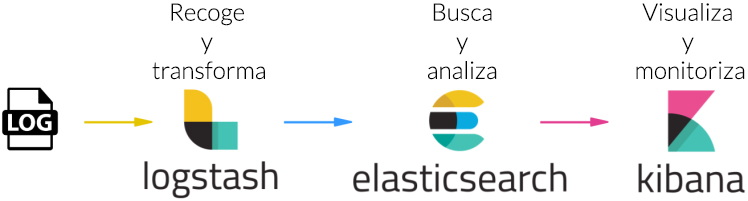
\includegraphics[width=1\linewidth]{img/elk.jpg}
    \caption{Arquitectura del sistema ELK.}
    \label{fig:elk}
\end{figure}
